% Compile with XeLaTeX. This file contains the contestant-facing statement only.
\documentclass[11pt,a4paper]{article}
\usepackage[margin=23mm,headheight=14pt]{geometry}
\usepackage{fontspec}
\setmainfont{Noto Serif CJK SC}[ItalicFont={Noto Serif CJK SC},ItalicFeatures={FakeSlant=0.15}]
\setsansfont{Noto Sans CJK SC}
\setmonofont{DejaVu Sans Mono}[Scale=0.86]
\XeTeXlinebreaklocale "zh"
\XeTeXlinebreakskip=0pt plus 1pt
\usepackage{amsmath,amssymb,booktabs,array,enumitem,tikz,fancyhdr,hyperref}
\usepackage{xurl}
\usetikzlibrary{arrows.meta,positioning}
\hypersetup{unicode=true,colorlinks=true,urlcolor=blue!50!black,linkcolor=black,
 pdftitle={低用水片区的余氯保障与有限排放},pdfauthor={SZUMMA2026 Training}}
\setlength{\parindent}{2em}
\setlength{\parskip}{4pt}
\setlist[enumerate]{leftmargin=2em,itemsep=5pt,topsep=4pt}
\pagestyle{fancy}
\fancyhf{}
\fancyhead[L]{\small 原创数学建模模拟题\quad Problem\_001}
\fancyhead[R]{\small 建议竞赛时长：96 小时}
\fancyfoot[C]{\thepage}
\renewcommand{\headrulewidth}{0.3pt}
\newcommand{\Cstar}{C_{\mathrm{tar}}}
\newcommand{\filepath}[1]{\texttt{\detokenize{#1}}}
\begin{document}
\begin{center}
{\LARGE\bfseries 低用水片区的余氯保障与有限排放}\par
\vspace{5pt}
{\small 原创训练题，非 CUMCM 或 MCM/ICM 官方赛题}
\end{center}

某供水片区原按较高入住率建设。节水措施和阶段性低入住率使用户用水明显减少，供水设施却不能随之缩小。水在管道和水箱中停留的时间变长，余氯可能不足。运行方可以从末梢排出部分水，使较新的水进入系统，但排放占用供水能力并消耗水资源，其效果还受到上游水体、设施混合和入口水质变化的影响。

运行方拟针对连续七天的低用水期制定管理方案：在有限排放预算下保障用户端余氯，并判断增加少量监测是否值得。请利用附件建立模型，为这一决策提供可检验的依据。题给片区、实验和运行记录均为\textbf{明确标识的合成训练数据}；其背景机制参考公开资料，数值不代表任何实际供水单位。

\section*{一、系统与运行条件}

系统拓扑如图。唯一入口为 $S$，$J$ 为体积可忽略的分流节点，$T_1,T_2$ 为在线水箱，$U_1,\ldots,U_6$ 为用户取水与可控排放位置。用户取水口与排放口处于同一末端位置，取用的是同一股水；排出的水不回用。管道编号、尺寸、有效附加耗氯率范围及认证流量上限见附件。

\begin{center}
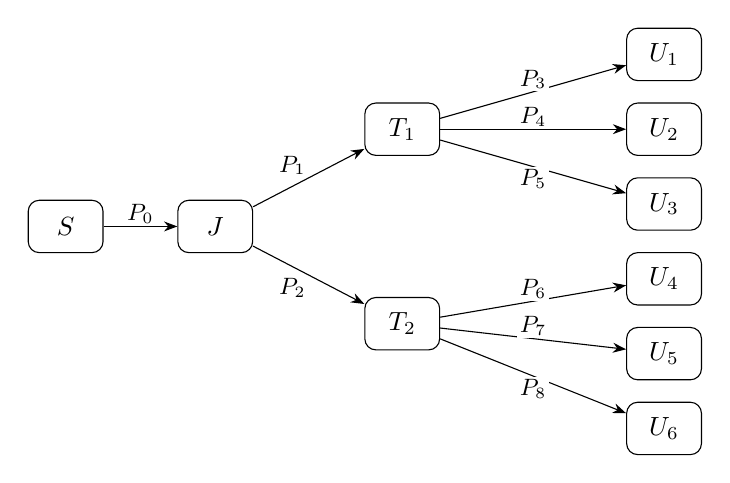
\begin{tikzpicture}[>=Stealth,scale=.95,every node/.style={transform shape},
 nd/.style={draw,rounded corners,minimum width=10mm,minimum height=7mm},
 lab/.style={font=\small,fill=white,inner sep=1pt}]
\node[nd] (s) at (0,0) {$S$};
\node[nd] (j) at (2,0) {$J$};
\node[nd] (t1) at (4.5,1.3) {$T_1$};
\node[nd] (t2) at (4.5,-1.3) {$T_2$};
\node[nd] (u1) at (8,2.3) {$U_1$};
\node[nd] (u2) at (8,1.3) {$U_2$};
\node[nd] (u3) at (8,.3) {$U_3$};
\node[nd] (u4) at (8,-.7) {$U_4$};
\node[nd] (u5) at (8,-1.7) {$U_5$};
\node[nd] (u6) at (8,-2.7) {$U_6$};
\draw[->] (s)--node[lab,above] {$P_0$}(j);
\draw[->] (j)--node[lab,above left] {$P_1$}(t1);
\draw[->] (j)--node[lab,below left] {$P_2$}(t2);
\draw[->] (t1)--node[lab,above] {$P_3$}(u1);
\draw[->] (t1)--node[lab,above] {$P_4$}(u2);
\draw[->] (t1)--node[lab,below] {$P_5$}(u3);
\draw[->] (t2)--node[lab,above] {$P_6$}(u4);
\draw[->] (t2)--node[lab,above] {$P_7$}(u5);
\draw[->] (t2)--node[lab,below] {$P_8$}(u6);
\end{tikzpicture}
\end{center}

研究期间持续保压且无倒流。每根管道始终充满水，其体积由几何尺寸确定。水箱通过补水装置保持固定水位，体积分别为 $18$ 和 $14\,\mathrm{m^3}$，每一时刻进流量与出流量相等；这并不意味着箱内水质均匀。节点没有其他取水、漏损、增压投药或换水操作。管道在指定方向上的流量由其下游用户需求与排放量确定。附件的流量上限已包含本题所需的供水能力约束，运行方确认在这些约束内可以保持压力；无需另外求解压力或水锤。

管内输运可以在横向充分混合、忽略轴向弥散的工程近似下研究，也可采用有依据的其他描述，但须检查其对结论的影响。本题只研究水体更新和余氯，不将排放视为除垢、去除生物膜或证明微生物安全的措施。水箱的附加壁面耗氯忽略；管道的附加耗氯范围见 \filepath{pipes.csv}，单位为 $\mathrm{h^{-1}}$，表示\textbf{整个管段中水体的有效一阶附加率}，不是单位管壁面积的反应系数。其温度修正因子约定为 $1.35^{(T-20)/5}$，不另乘几何系数。瓶试没有包含管壁作用。

以低用水期首日 00:00 为 $t=0$，时间单位为小时。附件给出 $[-72,168)$ 内的入口余氯、统一设施水温及用户名义需求，每行取值在对应的 $[h,h+1)$ 内保持不变。$[-72,0)$ 为此前正常用水期，$[0,168)$ 为决策期。水温是\textbf{各设施统一采用的水温工况}，不是仅入口水温；本题不要求建立传热模型。

为明确比较起点，统一假定 $t=-72$ 时全部设施充满水，余氯浓度为 $0.75\,\mathrm{mg/L}$，全部水体的初始水龄为 $12\,\mathrm{h}$。这是训练计算的初始状态，并非实测结论。之后从 $S$ 进入的水在进入时水龄为零，已有水体水龄随时间增长。\textbf{用户端平均水龄指该时刻用户取水中各水体水龄的平均值}，与箱内体积平均水龄须加以区分。正常用水期不进行额外排放。此前三天应参与状态计算，不应将 $t=0$ 的水体直接视为入口新水。

\section*{二、可用数据与排放约束}

附件中，瓶试是在避光、无管壁耗氯条件下，对两种初始余氯和三种恒定水温进行的独立试验。每组有三个独立平行瓶，第 1、2 瓶用于模型建立，第 3 瓶留作检验；同一瓶内各时点连续量测，不是独立实验重复。示踪试验则分别对两个水箱在恒定进出流量下进行：试验前示踪物为零，试验开始后入口归一化浓度从零跃为一，示踪物不反应。记录给出了箱出口的量测值及缺测标记；其中两个流量工况用于模型建立，一个较低流量工况留作检验。这些试验不包含整个管网的用户端余氯实测序列。合成机制公开，留出标签用于方法比较与数据使用记录，不构成保密盲测。生成说明和量测误差设定见数据说明，参赛队应明确哪些结论依赖额外假设。

每个末端均可自动排放。令 $u_i(h)$ 表示第 $h$ 小时在 $U_i$ 处的额外排放流量；开度在该小时内不变，允许连续取值。需要遵守以下条件：
\begin{enumerate}
\item $0\leq u_i(h)\leq2.2\,\mathrm{m^3/h}$，同一小时最多两个排放口开启。
\item 仅当地时钟 06:00 至 22:00 之前允许排放，即 $6\leq h\bmod24<22$；其余时段 $u_i(h)=0$。
\item 入口总流量不超过 $8\,\mathrm{m^3/h}$，各管道流量不超过附件上限。为预留需求误差的余量，制定每小时的排放动作时，必须按\textbf{该小时名义用户需求的 $1.25$ 倍}检验这些上限；排放流量本身不乘该系数。
\item 一周总排放量 $W=\sum_{h=0}^{167}\sum_{i=1}^{6}u_i(h)\,\Delta t$ 不超过给定预算 $B$，其中 $\Delta t=1\,\mathrm{h}$。需比较 $B=60,120,180\,\mathrm{m^3}$，并以 $B=0$ 为对照。
\end{enumerate}

用户原有需求不能被削减，也不能通过改变入口余氯实现本题的控制目标。运行方采用 $\Cstar=0.20\,\mathrm{mg/L}$ 作为本次训练的\textbf{服务目标}，不是对任一地区法规或完整饮水安全标准的替代。令 $d_i(t)$ 为用户取水流量，$C_i(t)$ 为用户取水处余氯。请至少报告以下指标，其中 $[x]_+=\max\{x,0\}$：
\begin{align*}
 D&=\int_0^{168}\sum_{i=1}^{6}d_i(t)\,dt,\\
 R&=\frac{\displaystyle\int_0^{168}\sum_{i=1}^{6}
 d_i(t)[\Cstar-C_i(t)]_+\,dt}{\Cstar D},\\
 F&=\frac{\displaystyle\int_0^{168}\sum_{i=1}^{6}
 d_i(t)\mathbf{1}_{\{C_i(t)<\Cstar\}}\,dt}{D}.
\end{align*}
这里 $R$ 为无量纲的需求加权余氯不足量，$F$ 为余氯低于目标的用户供水体积分数。另外报告每个末端在决策期内低于目标的\textbf{最长连续时段} $L_i$，单位为小时。排放水不得计入 $d_i$ 或 $D$，阈值交叉应采用足够细的时间尺度计算，并报告 $F,L_i$ 的数值精度与近阈值的不确定性。可提出补充指标，但须说明其必要性。

\newpage
\section*{三、研究任务}

\begin{enumerate}[label=\textbf{\arabic*.}]
\item \textbf{建立可检验的水质模型。}结合系统机制、瓶试与水箱示踪记录，建立能用于本片区预测的模型，比较模型复杂度与其对不同温度、初始余氯及流量条件的解释能力。按附件标签使用数据，以未参与模型建立的试验工况检查外推表现，说明现有数据能支持哪些性质，哪些仍不能确定。给出对余氯和水龄状态的必要描述，检查守恒、数值合理性和初始状态影响；不得仅凭瓶试确定管壁耗氯。

\item \textbf{评价低用水期的无排放运行。}预测各末端余氯随时间的变化，分析不足的时间、位置与成因，并报告上述指标及不确定性。某管理人员建议“以平均水龄对末端排序，并对平均水龄相同的水采用相同的余氯判断”。评价这一建议的可靠性，给出可检验的定量依据，说明它的适用条件和失效情形。说明低需求与正常需求之间的变化如何影响预测可信度。

\item \textbf{制定有限预算的排放方案。}在给定操作与容量约束下，为三个预算分别制定可执行的一周方案，分析水量投入、总体余氯保障与各末端连续不足之间的权衡。比较方案与无排放运行及一个合理、透明的简易管理方案；解释排放的作用时间与受益范围。若预算不能使所有末端全时段达到目标，应给出剩余不足和限制因素，不得将无法达标直接作为模型失败或通过忽略用户解决问题。评估关键假设和参数变化是否改变方案选择。

\item \textbf{评价监测与反馈的价值。}运行方最多增加两个余氯监测点，可选位置为 $J$、两箱出口及六个用户末端。位置在一周内固定；每点在时刻 $k=1,\ldots,168$ 读取瞬时余氯，零均值随机误差的标准差为 $0.01\,\mathrm{mg/L}$，可另有一周内固定、绝对值不超过 $0.015\,\mathrm{mg/L}$ 的偏差，随机误差分布由队伍说明。读数延迟一小时到达，不提供新增点的历史或 $t=0$ 读数。以 $B=120\,\mathrm{m^3}$ 为统一预算，设计监测配置和使用已收到信息的排放规则。与第三问相同预算的方案对照，在未用于策略设计的需求、耗氯及混合扰动情景中检验可靠性，至少覆盖三类扰动，并评价信息带来的收益与局限。需求、入口余氯和水温扰动界见 \filepath{operating_rules.json}，管壁耗氯范围见 \filepath{pipes.csv}；混合扰动及试验设计应有依据。请明确情景不是实际概率分布，也不得把同一模型中的闭环改善直接解释为现场成效。
\end{enumerate}

第四问的回放按整数小时推进。在时刻 $h$ 作决策时，可以使用全部名义预测、当前实际入口与统一水温、截至 $h-1$ 小时的实际用户取水量，以及此时已经到达的监测记录。附件全表为名义预测，未来实际扰动不可提前读取；在时刻 $k$ 采到的读数到 $k+1$ 才可使用，$k=168$ 的读数不用于本周决策。当前小时的实际需求和未来实际余氯不可提前读取，真实混合与耗氯参数也不直接告知控制器。对照与反馈方案使用相同初始状态和扰动情景，且均满足第二节约束。请记录策略的可用信息，验证未使用未来信息；检验系统与用于设计策略的模型至少在一项混合或反应假设上不同。

\newpage
\section*{四、附件与提交要求}

\begin{center}
\small
\begin{tabular}{p{.36\linewidth}p{.57\linewidth}}
\toprule
文件 & 内容\\
\midrule
\filepath{network_nodes.csv}、\filepath{pipes.csv} & 拓扑、几何、流量上限与附加耗氯范围\\
\filepath{tanks.csv}、\filepath{users.csv} & 箱容积、用户及排放口参数\\
\filepath{forcing.csv}、\filepath{demands.csv} & 三天正常期与七天低用水期的逐小时外部输入\\
\filepath{bottle_tests.csv} & 独立瓶试记录\\
\filepath{tank_tracer.csv} & 恒定流量水箱示踪记录、留出标签与缺测标记\\
\filepath{operating_rules.json} & 统一运行规则、初始状态与扰动界\\
\filepath{data/README.md} & 数据字典、合成说明与使用口径\\
\bottomrule
\end{tabular}
\end{center}
表中 CSV 和 JSON 文件均位于 \filepath{data/}。附件无需网络下载，公开生成程序用于数据复现，不构成指定解法。第三、四问的预测与策略结果由参赛队自行计算，附件不提供网络水质真值或预设最优方案。

提交一篇不超过 25 页的建模论文（含摘要、图表和参考文献），附主要程序及运行说明。论文应清楚给出假设、模型依据、验证方法、不确定性与结论的适用范围，避免用算法名称代替数学论证。另提交一页面向运行方的建议书；该页不计入论文页数。排放方案以 \filepath{time_h,user_id,flush_m3_h} 为字段提交 CSV，第三问每个预算各一份；第四问提供可回放的策略和监测配置说明。给出运行时间与软硬件条件。

\section*{背景参考资料}
\small
下列资料用于核查背景，不要求参赛队使用其中的软件或模型。附件的合成记录不来源于这些机构的实测数据。
\begin{enumerate}
\item US EPA. \emph{Protecting Water Quality Through Water Age Management}. 2022, EPA 815-F-22-002.\newline
\url{https://www.epa.gov/dwreginfo/drinking-water-distribution-system-tools-and-resources}
\item US EPA. \emph{Protecting Water Quality Through Distribution System Flushing}. 2022, EPA 815-F-22-003. 同上资料入口。
\item US EPA. \emph{Free Chlorine Distribution System Influent Hold Study Protocol}. 2019, EPA 815-B-19-013.\newline
\url{https://www.epa.gov/sdwa/free-chlorine-distribution-system-influent-hold-study-protocol}
\item US EPA. \emph{EPANET}.\newline
\url{https://www.epa.gov/water-research/epanet}
\end{enumerate}
\end{document}
